\normalfalse \difficiletrue \tdifficilefalse
\correctionfalse

%\UPSTIidClasse{11} % 11 sup, 12 spé
%\newcommand{\UPSTIidClasse}{12}

\exer{Pompe à pistons radiaux  $\star$ \label{C2:06:11}}
\setcounter{numques}{0}
\UPSTIcompetence{C2-06}
\index{Compétence C2-06}
\index{Pompe à pistons radiaux}
\index{Arbre à cames}
\ifcorrection
\else
\textbf{Pas de corrigé pour cet exercice.}
\fi

\ifprof
\else
Soit le mécanisme suivant. On a $\vect{AB}=e\vect{i_1}$ et $\vect{BI}=R\vect{j_0}$ et $\vect{AC}=\lambda(t)\vect{j_0}$. De plus, 
$e=\SI{10}{mm}$ et $R=\SI{20}{mm}$. Le contact entre \textbf{1} et \textbf{2} en $B$ est maintenu en permanence par un ressort suffisamment raide (non représenté) positionné entre \textbf{0} et \textbf{2}. 
\begin{center}
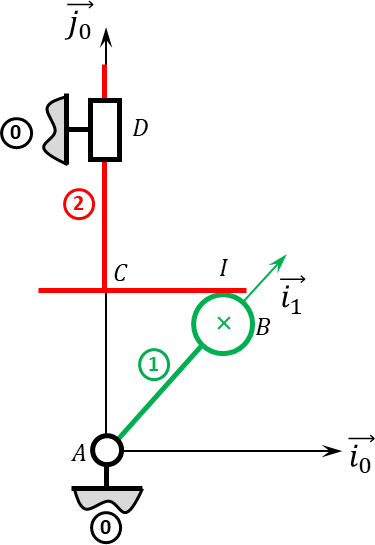
\includegraphics[width=\linewidth]{11_01}
\end{center}
\fi

\question{Tracer le graphe des liaisons.}
\ifprof
\else
\fi

\question{Exprimer $\lambda(t)$ en fonction de $\theta(t)$.}
\ifprof
\else
\fi

\question{Exprimer $\dot{\lambda}(t)$ en fonction de $\dot{\theta}(t)$.}
\ifprof
\else
\fi

\question{On note $S$ la section du piston \textbf{2}. Exprimer le débit instantané de la pompe.}
\ifprof
\else
\fi

\question{En utilisant Python, tracer le débit instantané de la pompe pour un tour de pompe pour $e=\SI{10}{mm}$ et $R=\SI{10}{mm}$ ainsi que pour $e=\SI{20}{mm}$ et $R=\SI{5}{mm}$. La fréquence de rotation est $\dot{\theta}(t)=\SI{100}{rad.s^{-1}}$, la section du piston est = $S=\SI{1}{cm^2}$.}
\ifprof
\else
\fi




\ifprof
\else
\begin{flushright}
\footnotesize{Corrigé  voir \ref{C2:06:11}.}
\end{flushright}%
\fi